\documentclass[14pt]{extarticle}
\usepackage{amsmath}
\usepackage{amssymb}
\usepackage{graphicx}
\graphicspath{ {../chap09/} }
\usepackage[top=1in, bottom=0.75in, left=0.75in, right=0.75in]{geometry}
\newcommand*{\Scale}[2][4]{\scalebox{#1}{\ensuremath{#2}}}%
\usepackage{hyperref}
\usepackage[most]{tcolorbox}
\definecolor{bg}{RGB}{255,249,227}


\begin{document}

\section*{Math208 Discussion Outline for 11/10/2020}

\subsection{Homework and other due dates}
\begin{itemize}
\item Section 9.5 due 11/10
\item Section 9.5, 9.7 due 11/13
\item Section 9.7 due 11/17
\item In class assignment due 11/15 \\\\
\resizebox{12cm}{!}{
	{When is the right time for Christmas music?}
}
\end{itemize}

\subsection{Questions?}
\begin{itemize}
	\item In lecture recordings, Professor Schultz covered 9.5 numbers 60, 78, 80, 82, 90 and 9.7 numbers 34, 36, 38, and 45.
\end{itemize}

\subsection{Goals}
\subsubsection*{Section 9.7: Marginal Analysis}
\begin{itemize}
	\item Recall and understand the business terminology
	\item Apply marginal analysis on costs revenues and profits
	\item Explain the results of your marginal analysis
\end{itemize}

\subsection{Warm up} Let $f(x) = 1/x  + x^2$ and $g(x)= (30 + x^2 - x^3)/x^2$, find:
\begin{align*}
	&\lim_{x \to -\infty}f(x)	&\lim_{x \to 0^-}f(x) \\\\
	&\frac{d}{dx}g(x)			&g'(3) 
\end{align*}
State the four step process for finding the deriviative of a function.


\cleardoublepage

\begin{center}
	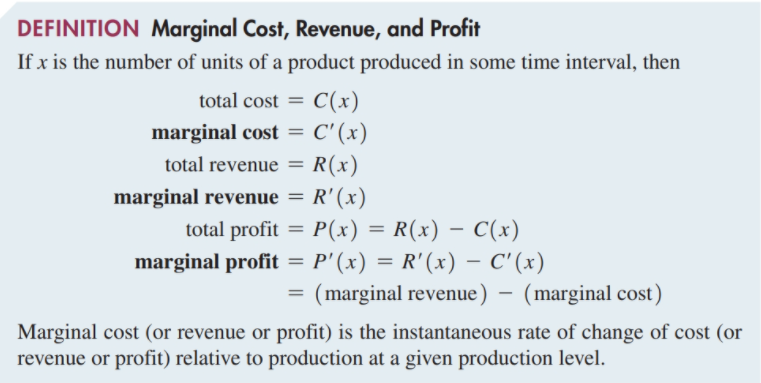
\includegraphics[width=0.9\linewidth]{9-7-1}
\end{center}

\begin{tcolorbox}[enhanced jigsaw,colback=bg,boxrule=0pt,arc=0pt]
	\textbf{Exact Cost, Revenue, and Profit}
	\begin{align*}
		\text{exact cost} &= C(x+1)-C(x) \\
		\text{exact revenue} &= R(x+1) - R(x) \\
		\text{exact profit} &= P(x+1) - P(x)
	\end{align*}
\end{tcolorbox}
\begin{center}
	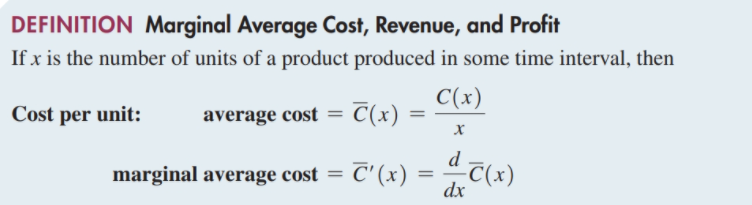
\includegraphics[width=0.9\linewidth]{9-7-2}
	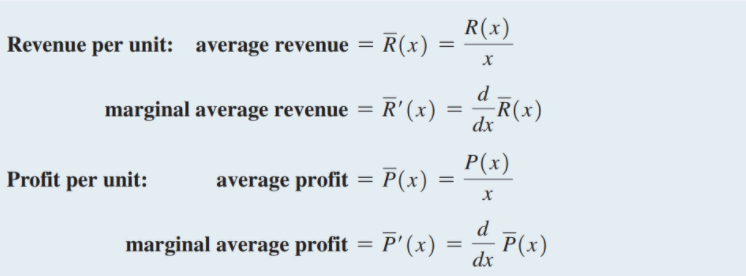
\includegraphics[width=0.9\linewidth]{9-7-3}
\end{center}

\cleardoublepage

\begin{center}
	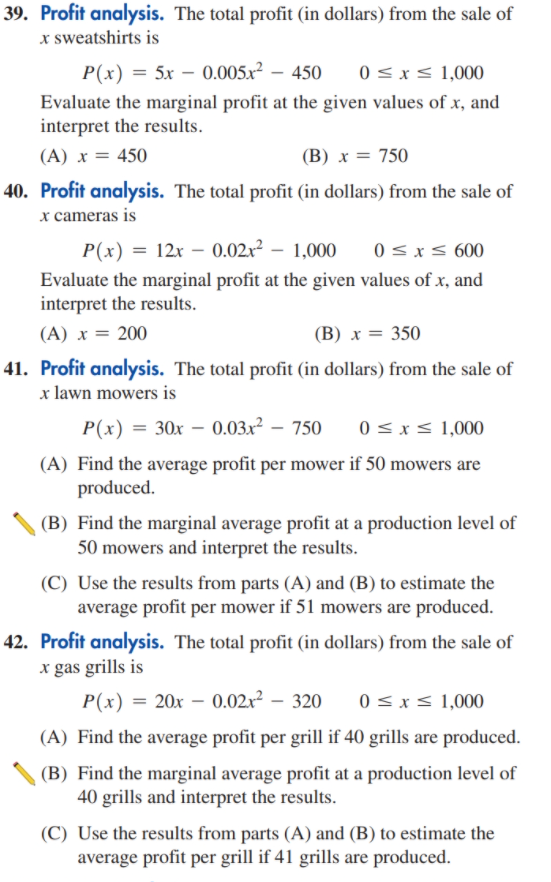
\includegraphics[width=0.8\linewidth]{9-7-4}
	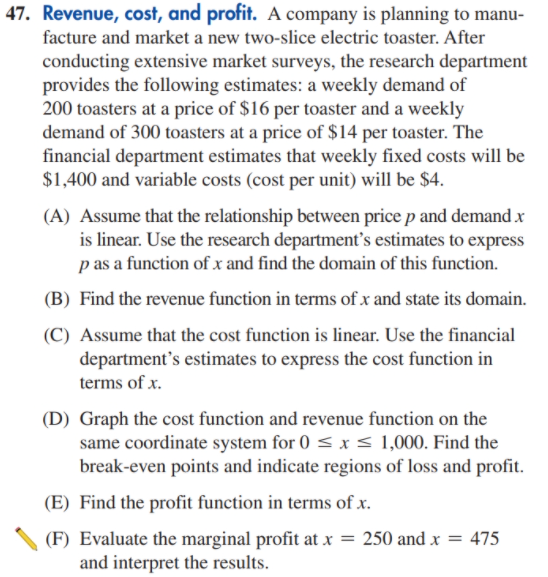
\includegraphics[width=0.8\linewidth]{9-7-5}
	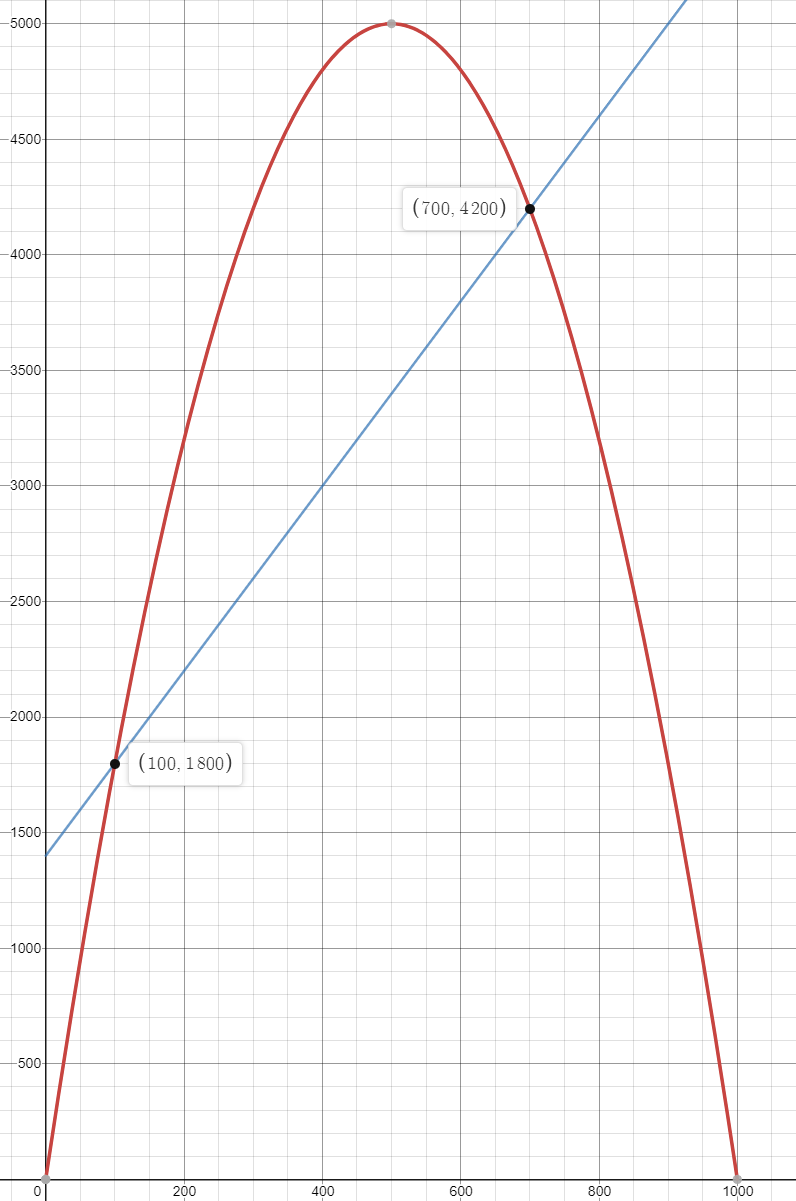
\includegraphics[width=0.9\linewidth]{9-7-6}
\end{center}





\end{document}
